\section{\Huge{32.3 XML-RPC}}

XML-RPC es uno de los protocolos de Servicios Web que citamos en el primer capítulo, y que se puede decir, 
de los más importantes, ya que Drupal lo soporta de manera nativa. Es decir, este protocolo está implementado 
en el Drupal sin necesitar módulos o librerías de la comunidad. En este capítulo, aprenderemos a trabajar con él 
y utilizarlo como un cliente y como un proveedor de Servicios Web.

\section{\Large{32.3.1 ¿Qué es XML-RPC?}}

Al igual que el protocolo SOAP visto anteriormente, XML-RPC se basa en RPC (\textit{Remote Procedure Call}), es decir, 
en llamadas a procedimientos remotos, para enviar y recibir mensajes cifrados en XML a través del protocolo HTTP.
Dichos mensajes contienen información sobre:

\begin{itemize}
  \item El procedimiento que se va a ejecutar en el servidor.
  \item Los parámetros
\end{itemize} 

Además, el servidor devuelve el resultado en formato XML.

\subsubsection{\large{Diferencias entre XML-RPC y SOAP}}

XML-RPC fue el primer mecanismo que surgió para invocar procedimientos remotos vía XML, ofrece una manera 
muy sencilla de invocar operaciones en sistemas heterogéneos a través de una estructura simple. Sin embargo, 
SOAP es una implementación más robusta para llevar acabo una intercomunicación en XML, a diferencia de XML-RPC 
a SOAP se le han integrado diversos mecanismos que le permiten operar en ambientes distribuidos mas complejos tales 
como:

\begin{itemize}
  \item Un lenguaje neutro para su descripción (WSDL/``Web Services Description Language'').
  \item Directorios distribuidos para su ubicación (UDDI/``Universal Discovery, Description and Integration'')  
\end{itemize} 

\subsubsection{\large{Prerrequisitos para XML-RPC}}

Si lo que queremos implementar es un servidor de peticiones, no tenemos que preocuparnos de ningún requisito previo, ya 
que al ser mensajes enviados a través de HTTP, utilizarán el puerto web estándar (puerto 80). El fichero \verb|xmlrpc.php| 
del directorio raíz de nuestro Drupal recibirá las peticiones y las enrutará.

Para ser usado como cliente, solo tenemos que tener en cuenta que muchas empresas de alojamiento Web no nos permiten 
realizar peticiones HTTP por razones de seguridad. Sería conveniente contactar con nuestro proveedor si no estamos seguros 
si nuestros clientes funcionarán.

\section{\Large{32.3.2 Drupal como servidor XML-RPC}}

Para configurar nuestro Drupal como un Servidor Web XML-RPC necesitaremos implementar tres puntos:

\begin{enumerate}
  \item Relación entre nombre de método remoto y función PHP a ejecutarse al ser llamados.
  \item La firma del método (\textit{signature}): tipo de retorno y de parámetros requeridos. Un método puede tener varias firmas.
  \item Documentación del método (\textit{docstring}).
\end{enumerate}

Como es normal en Drupal, vamos a implementar el ejemplo como un pequeño módulo que responda a peticiones. Procedemos pues a 
crear un ``Hola Mundo'' de un Servidor XML-RPC en Drupal, con la estructura y el código básicos. Para empezar, generaremos el 
fichero de información del módulo en \verb|sites/all/modules/holaxmlrpc/holaxmlrpc.info|:

\begin{verbatim}
name = Hola Mundo - Servidor XML RPC
description = Módulo que responderá con un "Hola" a cada petición XML-RPC 
				que se le realice a nuestro Drupal
package = Libro Experto Drupal 7
core = 7.x 
\end{verbatim}

El código de \verb|holaxmlrpc.module| quedaría como sigue:

\begin{verbatim}
<?php

/**
 * Implementacion del metodo hook_xmlrpc()
 * Relaciona nombre de procedimiento remoto y función PHP a ejecutarse
 */

function holaxmlrpc_xmlrpc()
{
    $metodos['remotoHola.hola'] = 'xmls_holaxmlrpc_hola';
    return $methodos;
}

/**
 * Saluda a una peticion
 * @param string $nombre
 */
function xmls_holaxmlrpc_hola($nombre) {
    if(!$nombre){
        return xmlrpc_error(1, t("Perdona, no te puedo saludar si no me dices tu nombre"));
    }
    return t("¡Hola, @nombre! ¿Que tal?", array("@nombre" => $nombre));
}
\end{verbatim}

¡Así de simple! Podemos complicar más nuestro servidor añadiendo más métodos en el array servicios de nuestro 
Drupal y validando los parámetros de entrada de las peticiones que se nos realizan. Primero veamos cómo funciona 
el \verb|hook\_xmlrpc()| y como testear este servicio.

Este \textit{hook} permite a un módulo registrar mapeos entre métodos de un Servicio Web y funciones de PHP 
a ejecutar, cuando un cliente invoca a los métodos de nuestro servidor XML-RPC. Devuelve un array con el mapeo así 
como configuración referida a la firma del método y la documentación del mismo. En nuestro ejemplo, el método 
\verb|remotoHola.hola| será el método público, y gracias a \verb|hook_xmlrpc()|, cada llamada a este método se 
manejará a través de la función PHP \verb|xmls_holaxmlrpc_hola()|. Normalmente se utiliza el prefijo \verb|xmls_|\footnote{
\textit{xmlns} es el atributo que se utiliza en XML para designar el espacio de nombres o \textit{namespace}} para las funciones 
PHP para indicar que esta función habla con el mundo exterior.

Además, podemos observar que en el código hemos útilizado un método para designar un error en la petición: 
\verb|xmlrpc_error()|, mediante el cual podemos indicar el código de error y el mensaje que se enviará al cliente. Los 
códigos de error son específicos de nuestra implementación, así que podremos utilizarlos a nuestro gusto.

Probemos nuestro servicio. Asumiendo que el módulo está alojado en un servidor \verb|ejemplo.com| y que nos 
encontramos en \verb|localhost|, tendremos que hacer una petición como la que sigue para comprobarlo:

\begin{verbatim}
$url = 'http://ejemplo.com/xmlrpc.php';
$nombre_metodo = 'remotoHola.hola';
$nombre = t('Fran');
$resultado = xmlrpc($url, array($nombre_metodo => array($nombre)));
\end{verbatim}

El resultado de ejecutar el código es:

\begin{verbatim}
echo $resultado;
>> (string) "¡Hola, Fran! ¿Que tal?"
\end{verbatim}

\subsubsection{\large{Firma y validación de los métodos}} 

Podemos, como mencionamos, validar los parámetros de entrada automáticamente utilizando el \verb|hook_xmlrpc()|. 
De esta manera, comprobaremos a nivel de servidor el mensaje que intentan enviarnos en la petición es correcto, sin 
añadir más lógica a nuestra función PHP final. Es muy recomendable utilizar esta validación, ya que Drupal 
se encargará de responder a las peticiones con respeto a nuestra firma de método, y si el mensaje no satisface 
lo descrito, será un método de Drupal (\verb|xmlrpc_server_call()|) el que responda con uno de los siguientes 
mensajes de error:
\begin{verbatim}
-32602: Server error. Invalid method parameters.
-32602: Server error. Wrong number of method parameters.
\end{verbatim}
dependiendo del caso.

La lista de todas las posibles validaciones de entrada se puede 
consultar en \verb|http://xmlrpc.scripting.com/spec.html|.

Veamos un ejemplo de cómo añadir la firma y validación a nuestro método:

\begin{verbatim}
/**
 * Implementacion del metodo hook_xmlrpc()
 * Relaciona nombre de procedimiento remoto y función PHP a ejecutarse
 */
function holaxmlrpc_xmlrpc() {
    $metodos = array();
    $metodos[] = array(
        'remotoHola.hola',         // Nombe de nuestro metodo externo
        'xmls_holaxmlrpc_hola',    // Funcion PHP a ejecutar
        array('string', 'String'), // Parametro de salida y despues, 
                                   // todos los tipos de parametros de entrada
        t('Saluda a clientes XML-RPC') // Descripcion
    );
    return $metodos;
}
\end{verbatim}

El siguiente diagrama nos servirá para mostarnos el ciclo de vida de una petición XML-RPC y para introducir términos 
relacionados con los métodos de sistema en XML-RPC:

\begin{figure}
  \centering
    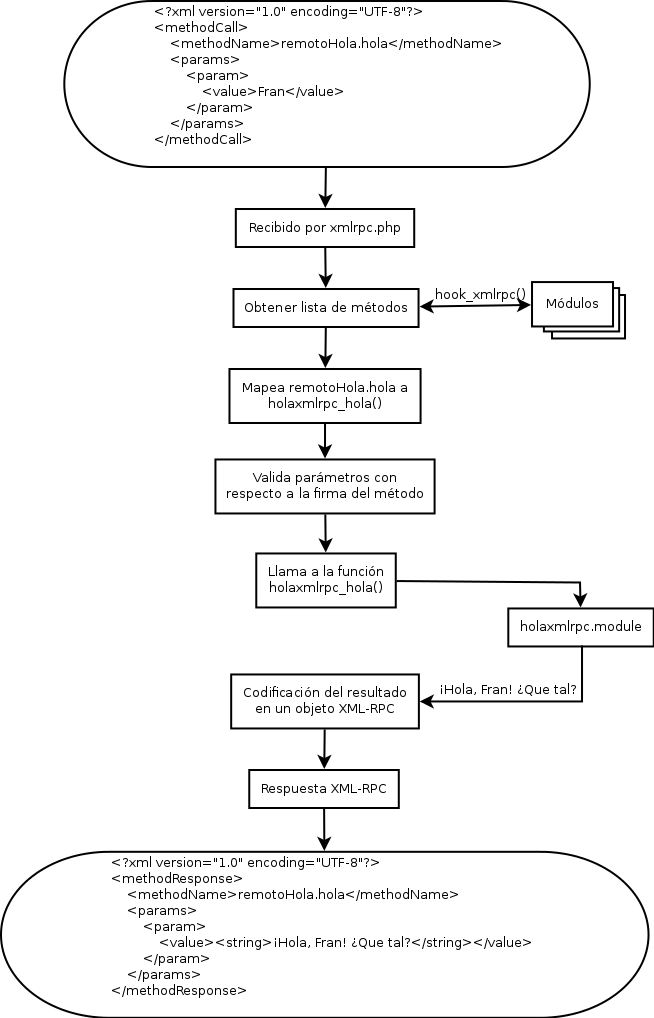
\includegraphics[width=1\textwidth]{Assets/xmlrpc/Imagenes/workflow.png}
  \caption{Diagrama de flujo de una petición XML-RPC}
\end{figure}

\section{\Large{32.3.3 Métodos XML-RPC de Drupal}}

Drupal tiene un listado de métodos de sistema para trabajar con XML-RPC como servidor. En este apartado describiremos 
cada uno de ellos.

\subsubsection{\large{system.listMethods}}

Se utiliza para listar todos los métodos disponibles de un Servidor XML-RPC. El método recorrerá todos los \verb|hook_xmlrpc()| 
de los módulos activos para obtener un array de dichos métodos.  Para realizar una petición, haremos algo como:

\begin{verbatim}
// Array con todos los métodos XML-RPC disponibles en el servidor
$url = 'http://ejemplo.com/xmlrpc.php';
$metodos = xmlrpc($url, array('system.listMethods'));
\end{verbatim}

La respuesta será un mensaje como el siguiente:

\begin{verbatim}
<?xml version="1.0" encoding="UTF-8"?>
<methodResponse>
    <params>
        <param>
            <value>
                <array>
                    <data>
                        <value>
                            <string>system.multiCall</string>
                        </value>
                        <value>
                            <string>system.methodSignature</string>
                        </value>
                        <value>
                            <string>system.getCapabilities</string>
                        </value>
                        <value>
                            <string>system.listMethods</string>
                        </value>
                        <value>
                            <string>system.methodHelp</string>
                        </value>
                        <value>
                            <string>remotoHola.hola</string>
                        </value>
                    </data>
                </array>
            </value>
        </param>
    </params>
</methodResponse>
\end{verbatim}

Así pues, ahora \verb|$metodos| contendrá un array con todos los métodos disponibles del sistema:

\begin{verbatim}
var_dump($metodos);
>> array('system.multicall', 'system.methodSignature',
		'system.getCapabilities', 'system.listMethods', 
		'system.methodHelp', 'remotoHola.hola')
\end{verbatim}

\subsubsection{\large{system.multiCall}}

Permite que se puedan realizar varias solicitudes XML-RPC en una sola llamada HTTP. Se le pasa una serie de 
llamadas XML-RPC codificadas de la siguiente manera:

\begin{verbatim}
{'methodName': nombreMetodo, 'params': arrayParametros}
\end{verbatim}

\subsubsection{\large{system.methodSignature}}

Este método nos permitirá consultar la firma de un método, es decir, todos los tipos de datos para los parámetros 
de entrada y el tipo del parámetro que devolverá la petición. Para recordar, nuestro servicio \verb|remotoHola.hola| 
tenía una salida de tipo \verb|string| y un parámetro de entrada de tipo \verb|string|.   	

Veamos cómo funciona:

\begin{verbatim}
// Obtiene la firma de un metodo
$url = 'http://ejemplo.com/xmlrpc.php';
$firma = xmlrpc($url, 'system.methodSignature', array('remotoHola.hola'));
\end{verbatim}

Esto devolverá:
\begin{verbatim}
var_dump($firma);
>> array('string', 'String');
\end{verbatim}

\subsubsection{\large{system.getCapabilities}}

Este método enumera todas las funciones que el servidor XML-RPC tiene, es decir, qué especificaciones están implementadas.
Drupal 7 implementa las siguientes especificaciones:

\begin{verbatim}
function xmlrpc_server_get_capabilities() {
  return array(
    'xmlrpc' => array(
      'specUrl' => 'http://www.xmlrpc.com/spec', 
      'specVersion' => 1,
    ), 
    'faults_interop' => array(
      'specUrl' => 'http://xmlrpc-epi.sourceforge.net/specs/rfc.fault_codes.php', 
      'specVersion' => 20010516,
    ), 
    'system.multicall' => array(
      'specUrl' => 'http://www.xmlrpc.com/discuss/msgReader$1208', 
      'specVersion' => 1,
    ), 
    'introspection' => array(
      'specUrl' => 'http://scripts.incutio.com/xmlrpc/introspection.html', 
      'specVersion' => 1,
    ),
  );
}
\end{verbatim}

\subsubsection{\large{system.methodHelp}}

Devuelve la descripción o \textit{docstring} del método XML-RPC, que es definido en el \verb|hook_xmlrpc()|. 
Para probarlo, se utiliza:

\begin{verbatim}
// Devuelve la descripción de un metodo
$url = 'http://ejemplo.com/xmlrpc.php';
$descripcion = xmlrpc($url, 'system.methodHelp', array('remotoHola.hola'));
\end{verbatim} 

El resultado de ejecución es:

\begin{verbatim}
var_dump($help);
>> (string) "Saluda a una peticion"
\end{verbatim}

\section{\Large{32.3.4 Drupal como cliente XML-RPC}}

Para realizar peticiones XML-RPC necesitaremos generar mensajes XML como se describió al principio de esta sección, 
utilizando los atributos \verb|<methodCall>| para indicar el tipo de mensaje, y el par de atributos \verb|<methodName>| 
y \verb|<params>| para hacer la llamada a un método utilizando una serie de parámetros.

Para trabajar creando un cliente, nos basaremos en un Servicio Web público para cálculos matemáticos:

\begin{verbatim}
http://www.cookcomputing.com/xmlrpcsamples/math.rem
\end{verbatim}

Si accedemos a la URL directamente, veremos los métodos implementados en este Servicio, así como la firma 
de cada uno (parámetros de entrada y salida). Utilizaremos el método \verb|xmlrpc()| para realizar una 
petición, por ejemplo al método \verb|Add|.

En Drupal, implementaremos la petición como:
 
\begin{verbatim}
$url = 'http://www.cookcomputing.com/xmlrpcsamples/math.rem';
$metodo = 'math.Add';
$parametros = array(1, 2);
$suma = xmlrpc($url, array($metodo => $parametros));
\end{verbatim}

Al ejectuarse este código, tendremos el siguiente resultado:

\begin{verbatim}
var_dump($suma);
>> (int) 3
\end{verbatim}

Para nosotros es realmente fácil trabajar de esta manera: no necesitamos construir mensajes XML, pero lo que 
realmente ocurre al lanzar el método \verb|xmlrpc()| es lo siguiente:

\begin{verbatim}
POST http://www.cookcomputing.com/xmlrpcsamples/math.rem
Content-Type: text/xml
<?xml version="1.0" encoding="UTF-8"?>
<methodCall>
    <methodName>math.Add</methodName>
    <params>
        <param>
            <value>
                <int>1</int>
            </value>
        </param>
        <param>
            <value>
                <int>2</int>
            </value>
        </param>
    </params>
</methodCall>
    

 -- response --
200 OK
Cache-Control:  private
Content-Type:  text/xml
Server:  Microsoft-IIS/7.0
X-AspNet-Version:  4.0.30319
X-Powered-By:  ASP.NET
Date:  Sun, 02 Sep 2012 10:07:15 GMT
Connection:  close
Content-Length:  161
<?xml version="1.0"?>
<methodResponse>
  <params>
    <param>
      <value>
        <i4>3</i4>
      </value>
    </param>
  </params>
</methodResponse>
\end{verbatim}

\subsubsection{\large{Manejo de Errores}}

La llamada que Drupal realiza por nosotros cuando ejecutabamos \verb|xmlrpc()| realmente la trata el método 
\verb|drupal_http_request()|. Por lo tanto, si tenemos un error desde nuestro servidor para acceder al Servicio, 
Drupal responderá con un error negativo, tal y como funciona en otros casos. Sabiendo esto, podemos comprobar 
en nuestro cliente si la petición puede ser ejecutada de la siguiente manera: 

\begin{verbatim}
$url = 'http://www.cookcomputing.com/xmlrpcsamples/math.rem';
$metodo = 'math.Add';
$parametros = array(1, 2);
$suma = xmlrpc($url, array($metodo => $parametros));
if ($error = xmlrpc_error()) {
    if ($error->code < 0) {
        $error->message = t("Host no alcanzable");
    }
    drupal_set_message(t("No se puede ejecutar el
    	calculo matematico: %message (@code)", 
            array('%message' => $error->message,
                     '@code' => $error->code)
            )
      );
}
\end{verbatim}

En caso de que no se pueda realizar la petición, obtendremos el siguiente mensaje en Drupal: 

\begin{verbatim}
No se puede ejecutar el calculo matematico: 
Host no alcanzable (-1827373)
\end{verbatim}

Para una petición no válida, si lo que está ocurriendo es que nuestro mensaje de envío no es válido, este trozo 
de código anterior nos responderá con el mensaje de error del Servidor. Veamos qué ocurre si intentamos 
utilizar un valor no válido con respecto a la firma del método, en este caso, una letra por un entero:

\begin{verbatim}
<?xml version="1.0" encoding="UTF-8"?>
<methodCall>
    <methodName>math.Add</methodName>
    <params>
        <param>
            <value>
                <string>a</string>
            </value>
        </param>
        <param>
            <value>
                <int>2</int>
            </value>
        </param>
    </params>
</methodCall>
\end{verbatim}

La respuesta será:

\begin{verbatim}
POST http://www.cookcomputing.com/xmlrpcsamples/math.rem
Content-Type: text/xml
<?xml version="1.0" encoding="UTF-8"?>
<methodCall>
    <methodName>math.Add</methodName>
    <params>
        <param>
            <value>
                <string>a</string>
            </value>
        </param>
        <param>
            <value>
                <int>2</int>
            </value>
        </param>
    </params>
</methodCall>
    

 -- response --
200 OK
Cache-Control:  private
Content-Type:  text/xml
Server:  Microsoft-IIS/7.0
X-AspNet-Version:  4.0.30319
X-Powered-By:  ASP.NET
Date:  Sun, 02 Sep 2012 10:53:16 GMT
Connection:  close
Content-Length:  492
<?xml version="1.0"?>
<methodResponse>
  <fault>
    <value>
      <struct>
        <member>
          <name>faultCode</name>
          <value>
            <i4>0</i4>
          </value>
        </member>
        <member>
          <name>faultString</name>
          <value>
            <string>Object of type 'System.String' 
            cannot be converted to type 'System.Int32'.</string>
          </value>
        </member>
      </struct>
    </value>
  </fault>
</methodResponse>
\end{verbatim}

Y nuestro Drupal responderá con:

\begin{verbatim}
No se puede ejecutar el calculo matematico debido a 
Object of type 'System.String' cannot be converted 
to type 'System.Int32'. (0)
\end{verbatim}



